\documentclass[letterpaper,12pt]{article}
\usepackage{array}
\usepackage{threeparttable}
\usepackage{geometry}
\geometry{letterpaper,tmargin=1in,bmargin=1in,lmargin=1.25in,rmargin=1.25in}
\usepackage{fancyhdr,lastpage}
\pagestyle{fancy}
\lhead{}
\chead{}
\rhead{}
\lfoot{}
\cfoot{}
\rfoot{\footnotesize\textsl{Page \thepage\ of \pageref{LastPage}}}
\renewcommand\headrulewidth{0pt}
\renewcommand\footrulewidth{0pt}
\usepackage[format=hang,font=normalsize,labelfont=bf]{caption}
\usepackage{listings}
\usepackage{color}
\definecolor{dkgreen}{rgb}{0,0.6,0}
\definecolor{gray}{rgb}{0.5,0.5,0.5}
\definecolor{mauve}{rgb}{0.58,0,0.82}
\lstset{ %
  language=R,                     % the language of the code
  basicstyle=\footnotesize,       % the size of the fonts that are used for the code
  numbers=left,                   % where to put the line-numbers
  numberstyle=\tiny\color{gray},  % the style that is used for the line-numbers
  stepnumber=1,                   % the step between two line-numbers. If it's 1, each line
  numbersep=5pt,                  % how far the line-numbers are from the code
  backgroundcolor=\color{white},  % choose the background color. You must add \usepackage{color}
  showspaces=false,               % show spaces adding particular underscores
  showstringspaces=false,         % underline spaces within strings
  showtabs=false,                 % show tabs within strings adding particular underscores
  frame=single,                   % adds a frame around the code
  rulecolor=\color{black},        % if not set, the frame-color may be changed on line-breaks within not-black text (e.g. commens (green here))
  tabsize=2,                      % sets default tabsize to 2 spaces
  captionpos=b,                   % sets the caption-position to bottom
  breaklines=true,                % sets automatic line breaking
  breakatwhitespace=false,        % sets if automatic breaks should only happen at whitespace
  title=\lstname,                 % show the filename of files included with \lstinputlisting;
  keywordstyle=\color{blue},      % keyword style
  commentstyle=\color{dkgreen},   % comment style
  stringstyle=\color{mauve},      % string literal style
  escapeinside={\%*}{*)},         % if you want to add a comment within your code
  morekeywords={*,...}            % if you want to add more keywords to the set
}
\usepackage{amsmath}
\usepackage{amssymb}
\usepackage{amsthm}
\usepackage{harvard}
\usepackage{setspace}
\usepackage{float,color}
\usepackage[pdftex]{graphicx}
\usepackage{hyperref}
\hypersetup{colorlinks,linkcolor=red,urlcolor=blue}
\theoremstyle{definition}
\newtheorem{theorem}{Theorem}
\newtheorem{acknowledgement}[theorem]{Acknowledgement}
\newtheorem{algorithm}[theorem]{Algorithm}
\newtheorem{axiom}[theorem]{Axiom}
\newtheorem{case}[theorem]{Case}
\newtheorem{claim}[theorem]{Claim}
\newtheorem{conclusion}[theorem]{Conclusion}
\newtheorem{condition}[theorem]{Condition}
\newtheorem{conjecture}[theorem]{Conjecture}
\newtheorem{corollary}[theorem]{Corollary}
\newtheorem{criterion}[theorem]{Criterion}
\newtheorem{definition}[theorem]{Definition}
\newtheorem{derivation}{Derivation} % Number derivations on their own
\newtheorem{example}[theorem]{Example}
\newtheorem{exercise}[theorem]{Exercise}
\newtheorem{lemma}[theorem]{Lemma}
\newtheorem{notation}[theorem]{Notation}
\newtheorem{problem}[theorem]{Problem}
\newtheorem{proposition}{Proposition} % Number propositions on their own
\newtheorem{remark}[theorem]{Remark}
\newtheorem{solution}[theorem]{Solution}
\newtheorem{summary}[theorem]{Summary}
%\numberwithin{equation}{section}
\bibliographystyle{aer}
\newcommand\ve{\varepsilon}
\newcommand\boldline{\arrayrulewidth{1pt}\hline}


\begin{document}

\begin{flushleft}
  \textbf{\large{Problem Set \#2}} \\
  MACS 30100, Dr. Evans \\
  Cheng Yee Lim
\end{flushleft}

\vspace{5mm}

\noindent\textbf{Problem 1}\\
\textbf{Part (a).}
\begin{figure}[htb]\centering\captionsetup{width=4.0in}
  \caption{\textbf{Density histogram of Annual Incomes of MACSS Graduates}}\label{FigExample}
  \fbox{\resizebox{6.0in}{4.0in}{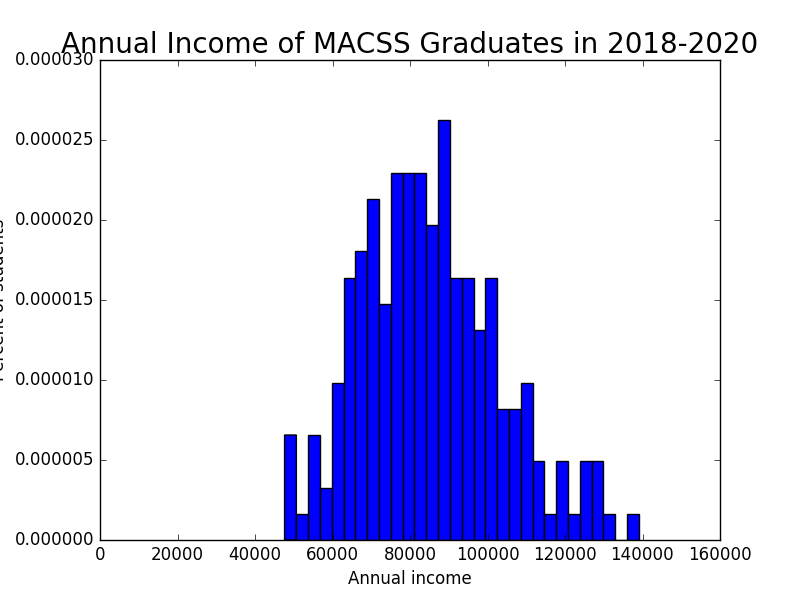
\includegraphics{images/1a.png}}}
\end{figure}

\pagebreak
\textbf{Part (b).} \\
\begin{figure}[htb]\centering\captionsetup{width=4.0in}
  \caption{\textbf{Density histogram of Annual Incomes of MACSS Graduates}}\label{FigExample}
  \fbox{\resizebox{6.0in}{4.0in}{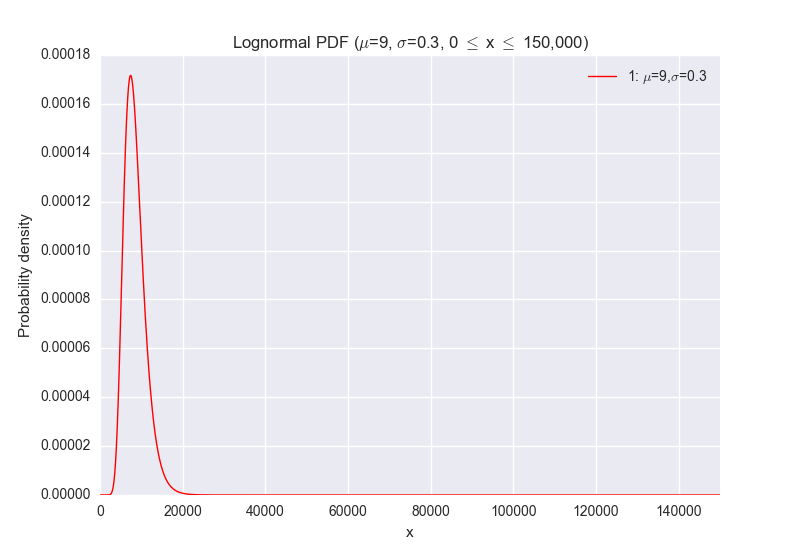
\includegraphics{images/1b.png}}}
\end{figure}

\flushleft The log likelihood value for the parameters $\mu$ = 9 and $\sigma$ = 0.3 is -8298.64. The very negative log likelihood value suggests that this parameters are a bad fit for the data given. 
\flushleft

\textbf{Part (c).} \\
\begin{figure}[htb]\centering\captionsetup{width=4.0in}
  \caption{\textbf{Normed Histogram of MACSS Students Annual Income and Log PDFs}}\label{FigExample}
  \fbox{\resizebox{6.0in}{4.0in}{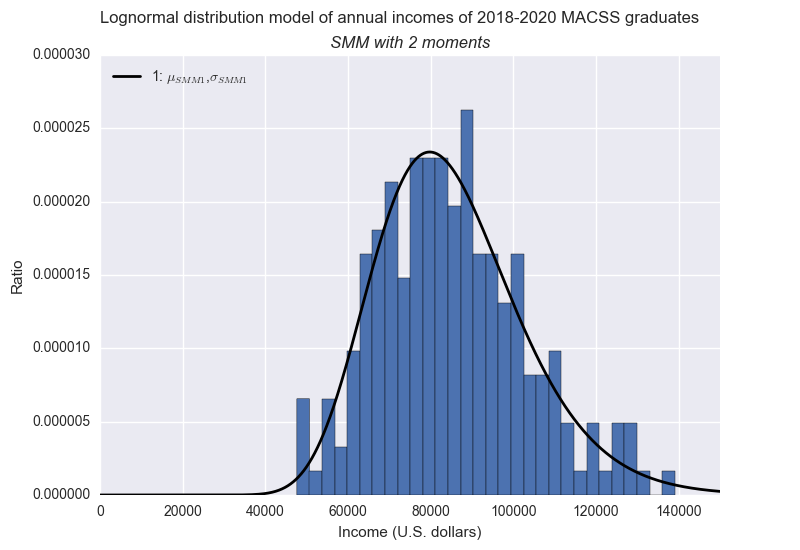
\includegraphics{images/1c.png}}}
\end{figure}
\flushleft 
The ML estimates for $\mu$ and $\sigma$ are 11.331 and 0.212. 

\flushleft 
The log likelihood value for $\mu$ = 11.331 and $\sigma$ = 0.212 is -2239.534744. The log likelihood value is much less negative than log likelihood value in part (b). This proves that the ML estimates for $\mu$ and $\sigma$ are a better fit for the data given than the parameters in part (b).

\flushleft 
The variance-covariance matrix, $M_1$, is reported below. 
\[
M_1 =
  \begin{bmatrix}
    2.73\times 10^{-4} &  1.55\times10^{-6}  \\
    1.55\times 10^{-6} &  1.11\times10^{-4} 
  \end{bmatrix}
\]

\flushleft

\pagebreak
\textbf{Part (d).} \\
\flushleft 
According to the likelihood ratio test, there is no probability that the data in incomes.txt came from the distribution in part (b). 

\flushleft

\textbf{Part (e).} \\
\flushleft Using the estimated model from part (c), the probability of a MACSS graduate will earn more than \$100,000 annually is 0.196 and the probability of a MACSS graduate earning less than \$75,000 is 0.308. 

\flushleft


\newpage
\noindent\textbf{Problem 2}\\
\textbf{Part (a).} \\
\flushleft 
\begin{equation}
sick_{i}=\beta_0+\beta_1age_{i}+\beta_2children_i+\beta_3temp\_winter_{i}+\varepsilon_{i}
\end{equation}
\begin{equation}
where\quad \varepsilon_i \texttt{\char`\~} N(0, \sigma^2)\nonumber
\end{equation}
To solve the parameters $(\beta_0, \beta_1, \beta_2, \beta_3, \sigma)$ of model (1), we leverage on the fact that the error term is normally distributed at $\mu$ = 0 and solve the regression equation for $\varepsilon_i$

\begin{equation}
\varepsilon_{i}= sick_i - \beta_0 - \beta_1age_{i}-\beta_2children_i-\beta_3temp\_winter_{i}
\end{equation}

The estimates for the parameters of the model are as follows: 
$\beta_0$ = 0.25164638, $\beta_1$ = 0.01293335, $\beta_2$ = 0.40050205, $\beta_3$ = -0.00999167,  $\sigma$ = 0.00301768

\flushleft 
The value of the log likelihood function is 876.865046288.

\flushleft 
The variance-covariance matrix, $M_2$, is reported below. 
\[
M_2 =
  \begin{bmatrix}
1 &  0&  0&  0&  0\\
0 &  1&  0&  0&  0\\
0 &  0&  1&  0&  0\\
0 &  0&  0&  1&  0\\
0 &  0&  0&  0&  1\\
\end{bmatrix}
\]


\textbf{Part (b).} \\
\flushleft 
The probability that $\beta_0$ = 1.0, $\sigma^2$ = 0.01 and $\beta_1, \beta_2, \beta_3$ = 0 is 0.00. The likelihood that age, number of children, and average winter temperature have no effect on the number of sick days is 0. The conclusion is highly probable as people fall sick more easily when the winter is colder, and more children means more exposure to germs from people they interact with.  
\end{document}
